\section{Introduction}
\begin{frame}{Introduction}
  \begin{itemize}
  \item Smart grids are becoming a necessity in order to integrate renewables, accommodate new actors, improve the observability and efficiency.
    \item The transition from conventional systems towards smart grids is challenging:
      \begin{itemize}
        \item Incorporate distributed sources of energy.
        \item Integrate storage systems.
        \item Rely less on large traditional centralized power plants.
      \end{itemize}
  \end{itemize}
  Thus, we have divided the progressive adaptations:
  \begin{table}\footnotesize
    \begin{tabular}{cc}
      \hline
      \textbf{Chapter} & \textbf{Activities} \\
      \hline
      \hline
      Phase 1 & Initial solution of the system \\
      Phase 2 & Addition of lines \\
      Phase 3 & Integration of wind and solar \\
      Phase 4 & Rehabilitated power plant and storage \\
      SGAM & HLUC related to contingencies \\
      \hline
    \end{tabular}
    \caption{Phases of the project to move towards smart grids}
  \end{table}
\end{frame}


\AtBeginSection[]
  {
     \begin{frame}<beamer>
     \frametitle{Plan}
     \tableofcontents[currentsection]
     \end{frame}
  }



\section{Phase 1}
\begin{frame}{System overview}


\begin{figure}[!htb]\centering

  \resizebox{8.0cm}{7cm}{
  \begin{circuitikz}[/tikz/circuitikz/bipoles/length=1cm, line width=0.8pt]

    % grid
    \draw[gray!50!white, line width=0.5pt] (0.0,0.0) to [short] (8.0,0.0);
    \draw[gray!50!white, line width=0.5pt] (0.0,1.6) to [short] (8.0,1.6);
    \draw[gray!50!white, line width=0.5pt] (0.0,3.2) to [short] (8.0,3.2);
    \draw[gray!50!white, line width=0.5pt] (0.0,4.8) to [short] (8.0,4.8);
    \draw[gray!50!white, line width=0.5pt] (0.0,6.4) to [short] (8.0,6.4);
    \draw[gray!50!white, line width=0.5pt] (0.0,8.0) to [short] (8.0,8.0);

    \draw[gray!50!white, line width=0.5pt] (0.0,0.0) to [short] (0.0,8.0);
    \draw[gray!50!white, line width=0.5pt] (1.6,0.0) to [short] (1.6,8.0);
    \draw[gray!50!white, line width=0.5pt] (3.2,0.0) to [short] (3.2,8.0);
    \draw[gray!50!white, line width=0.5pt] (4.8,0.0) to [short] (4.8,8.0);
    \draw[gray!50!white, line width=0.5pt] (6.4,0.0) to [short] (6.4,8.0);
    \draw[gray!50!white, line width=0.5pt] (8.0,0.0) to [short] (8.0,8.0);


    % generators
    \draw (3.2,-1.8) to [sV, fill=magenta!70!cyan] (3.2,-1.2);
    \draw [short] (3.2,-1.2) to [short] (3.2,-1.0);
    \draw (-1.8,1.6) to [sV, fill=green!50!white] (-1.2,1.6);
    \draw [short] (-1.2,1.6) to [short] (-1.0,1.6);
    \draw (9.2,1.6) to [sV, fill=cyan!50!white] (9.8,1.6);
    \draw [short] (9.2,1.6) to [short] (9.0,1.6);
    \draw (4.8,3.6) to [sV, fill=black!60!white] (4.8,3.0);
    \draw [short] (4.8,3.6) to [short] (4.8,3.8);
    \draw (8.4,4.8) to [sV, fill=yellow!60!white] (9.0,4.8);
    \draw [short] (8.0,4.8) to [short] (8.4,4.8);
    \draw (1.6,9.2) to [sV, fill=orange!60!white] (1.6,9.8);
    \draw [short] (1.6,9.0) to [short] (1.6,9.2);


    % large buses
    \draw[line width=2.5pt] (2.7,0) to [short] (3.7,0);
    \draw[line width=2.5pt] (0.0,1.1) to [short] (0,2.1);
    \draw[line width=2.5pt] (8.0,1.1) to [short] (8,2.1);
    \draw[line width=2.5pt] (1.1,8) to [short] (2.1,8);
    \draw[line width=2.5pt] (2.7,3.2) to [short] (3.7,3.2);
    \draw[line width=2.5pt] (2.7,4.8) to [short] (3.7,4.8);
    \draw[line width=2.5pt] (4.3,6.4) to [short] (5.3,6.4);
    \draw[line width=2.5pt] (0.0,5.9) to [short] (-0.0,6.9);
    \draw[line width=2.5pt] (8,4.3) to [short] (8,5.3);
    \draw[line width=2.5pt] (4.3,4.8) to [short] (5.3,4.8);

    % small buses
    \draw[line width=2.5pt] (2.9,-1) to [short] (3.5,-1);
    \draw[line width=2.5pt] (-1.0,1.3) to [short] (-1,1.9);
    \draw[line width=2.5pt] (9,1.3) to [short] (9,1.9);
    \draw[line width=2.5pt] (4.5,3.8) to [short] (5.1,3.8);
    \draw[line width=2.5pt] (1.3,9.0) to [short] (1.9,9.0);

    \draw[line width=2.5pt] (1.75,3.2) to [short] (1.75,2.6);
    \draw[line width=2.5pt] (1.75,4.8) to [short] (1.75,4.2);
    \draw[line width=2.5pt] (-0.95,6.7) to [short] (-0.95,6.1);
    \draw[line width=2.5pt] (4.5,7.35) to [short] (5.1,7.35);

    % trafos
    \draw (3.2,-1.0) to [voosource] (3.2,0.0);
    \draw (-1,1.6) to [voosource] (0,1.6);
    \draw (8,1.6) to [voosource] (9,1.6);
    \draw (1.6,8) to [voosource] (1.6,9);
    \draw (4.8,4.8) to [voosource] (4.8,3.8);

    \draw (-1,6.4) to [voosource] (0,6.4);
    \draw (4.8,6.4) to [voosource] (4.8,7.4);
    \draw (2.7,4.5) to [voosource] (1.7,4.5);
    \draw (2.7,2.9) to [voosource] (1.7,2.9);

    % loads
    \draw[-{Triangle[length=5mm, width=2mm]}, draw=blue!60!white, fill=blue!60!white] (-1,6.4) -- (-1.6,6.4);
    \draw[-{Triangle[length=5mm, width=2mm]}, draw=blue!60!white, fill=blue!60!white] (4.8,7.4) -- (4.8,8.0);
    \draw[-{Triangle[length=5mm, width=2mm]}, draw=red!60!white, fill=red!60!white] (1.7,4.5) -- (1.1,4.5);
    \draw[-{Triangle[length=5mm, width=2mm]}, draw=blue!60!white, fill=blue!60!white] (1.7,2.9) -- (1.1,2.9);

    \draw (3.0,4.8) to [short] (3.0,4.5);
    \draw (3.0,4.5) to [short] (2.7,4.5);

    \draw (3.0,3.2) to [short] (3.0,2.9);
    \draw (3.0,2.9) to [short] (2.7,2.9);

    % lines
    \draw (3.15,0) to [short] (3.15,3.2);
    \draw (3.25,0) to [short] (3.25,3.2);
    \draw (3.15,3.2) to [short] (3.15,4.8);
    \draw (3.25,3.2) to [short] (3.25,4.8);
    \draw (4.6,4.8) to [short] (4.6,5.1);
    \draw (4.6,5.1) to [short] (3.4,5.1);
    \draw (3.4,5.1) to [short] (3.4,4.8);
    \draw (3.15,4.8) to [short] (3.15,5.1);
    \draw (3.25,4.8) to [short] (3.25,5.1);
    \draw (3.15,5.1) to [short] (4.55,6.1);
    \draw (3.25,5.1) to [short] (4.65,6.1);
    \draw (4.55,6.1) to [short] (4.55,6.4);
    \draw (4.65,6.1) to [short] (4.65,6.4);
    \draw (5.0,6.4) to [short] (5.0,6.1);
    \draw (5.0,6.1) to [short] (7.7,5.1);
    \draw (7.7,5.1) to [short] (8.0,5.1);
    \draw (0,6.4) to [short] (0.3,6.4);
    \draw (0.3,6.4) to [short] (3.0,5.1);
    \draw (3.0,5.1) to [short] (3.0,4.8);


    % legend
    \draw[-{Triangle[length=5mm, width=2mm]}, draw=blue!60!white, fill=blue!60!white] (3.0,8.4) -- (4.0,8.4);
    \draw[-{Triangle[length=5mm, width=2mm]}, draw=red!60!white, fill=red!60!white] (3.0,9.1) -- (4.0,9.1);
    \draw (3.2,9.8) to [sV, fill=magenta!70!cyan] (3.8,9.8);

    \draw (6.0,9.8) to [sV, fill=black!60!white] (6.6,9.8);
    \draw (6.0,9.1) to [sV, fill=yellow!60!white] (6.6,9.1);
    \draw (6.0,8.4) to [sV, fill=green!50!white] (6.6,8.4);

    \draw (9.0,9.8) to [sV, fill=orange!60!white] (9.6,9.8);
    \draw (9.0,9.1) to [sV, fill=cyan!50!white] (9.6,9.1);

    \node at (4.73, 9.8) {\footnotesize Nuclear};
    \node at (4.66, 9.1) {\footnotesize Load I};
    \node at (4.72, 8.4) {\footnotesize Load II};

    \node at (7.64, 9.8) {\footnotesize Dismantled};
    \node at (7.49, 9.1) {\footnotesize Intercon.};
    \node at (7.28, 8.4) {\footnotesize Wind};

    \node at (10.25, 9.8) {\footnotesize Solar};
    \node at (10.40, 9.1) {\footnotesize Storage};

    \draw[gray!50!white, line width=0.5pt] (8.5,8.0) to [short] (10.1,8.0);
    \draw[gray!50!white, line width=0.5pt] (8.5,6.4) to [short] (10.1,6.4);
    \draw[gray!50!white, line width=0.5pt] (8.5,6.4) to [short] (8.5,8.0);
    \draw[gray!50!white, line width=0.5pt] (10.1,6.4) to [short] (10.1,8.0);

    \node at (9.30, 6.2) {\footnotesize 50 km};
    \node[rotate=90] at (10.3, 7.2) {\footnotesize 50 km};

    \draw [fill=gray, opacity=0.2, line width=0.01pt] (2.95,10.15) rectangle (11.0,8.05);
    \draw [fill=gray, opacity=0.2, line width=0.01pt] (11.0,8.05) rectangle (8.05,6.05);

    % buses nodes and labels
    \node at (3.6, 0.2) {8};
    \node at (3.6, -1.0) {1};
    \node at (3.6, 4.6) {9};
    \node at (1.5, 4.75) {2};
    \node at (3.6, 3.0) {10};
    \node at (1.5, 3.15) {3};
    \node at (4.4, 6.6) {11};
    \node at (4.4, 7.6) {4};
    \node at (0.2, 6.7) {12};
    \node at (-1.2, 6.7) {5};
    \node at (5.2, 4.6) {13};
    \node at (5.3, 3.8) {7};
    \node at (7.8, 4.6) {6}; 



\end{circuitikz}}

  \caption{Overview of the network}
  \label{fig:net1}
\end{figure}

\end{frame}

\subsection{Results}
\begin{frame}{Initial bus voltages}

\begin{figure}[!htb]\centering
  \resizebox{12cm}{6cm}{
\begin{tikzpicture}
    \begin{axis}[xlabel={Hour}, ylabel={$|V|$ (p.u.)}, grid=both, grid style={line width=.1pt, draw=gray!10}, major grid style={line width=.2pt,draw=gray!50}, xtick distance = 2, ytick distance = 0.02, width=12cm, height=8cm, every plot/.append style={very thick}, xmin = 1, xmax = 24, ymin=0.8, very thick, grid=both, grid style={line width=.4pt, draw=gray!10}, major grid style={line width=.8pt,draw=gray!50}, legend style={at={(1.03,0.14)},anchor=south west}]
        \addplot[color=magenta] table[col sep=comma, x=x, y=y1] {Data/phase1/ph1_vpu.csv};
        \addplot[color=red] table[col sep=comma, x=x, y=y2] {Data/phase1/ph1_vpu.csv};
        \addplot[color=green] table[col sep=comma, x=x, y=y3] {Data/phase1/ph1_vpu.csv};
        \addplot[color=cyan] table[col sep=comma, x=x, y=y4] {Data/phase1/ph1_vpu.csv};
        \addplot[color=blue] table[col sep=comma, x=x, y=y5] {Data/phase1/ph1_vpu.csv};
        \addplot[color=orange, dashed] table[col sep=comma, x=x, y=y6] {Data/phase1/ph1_vpu.csv};
        \addplot[color=magenta, dashed] table[col sep=comma, x=x, y=y8] {Data/phase1/ph1_vpu.csv};
        \addplot[color=red, dashed] table[col sep=comma, x=x, y=y9] {Data/phase1/ph1_vpu.csv};
        \addplot[color=green, dashed] table[col sep=comma, x=x, y=y10] {Data/phase1/ph1_vpu.csv};
        \addplot[color=cyan, dashed] table[col sep=comma, x=x, y=y11] {Data/phase1/ph1_vpu.csv};
        \addplot[color=blue, dashed] table[col sep=comma, x=x, y=y12] {Data/phase1/ph1_vpu.csv};
\legend{Bus 1, Bus 2, Bus 3, Bus 4, Bus 5, Bus 6, Bus 8, Bus 9, Bus 10, Bus 11, Bus 12};
\end{axis}
\end{tikzpicture}}
    \caption{Voltage profile during 24 hours for the initial grid. The low-voltage buses are plotted in solid lines; the high-voltage ones are in dashed lines.}
    \label{fig:vpu_ph1}
  \end{figure}

\end{frame}

\begin{frame}{Initial lines loading}


\begin{figure}[!htb]\centering
  \resizebox{12cm}{5.9cm}{
\begin{tikzpicture}
    \begin{axis}[xlabel={Hour}, ylabel={Load (\%)}, grid=both, grid style={line width=.1pt, draw=gray!10}, major grid style={line width=.2pt,draw=gray!50}, xtick distance = 2, ytick distance = 10, width=12cm, height=8cm, every plot/.append style={very thick}, xmin = 1, xmax = 24, ymin=0.0, very thick, grid=both, grid style={line width=.4pt, draw=gray!10}, major grid style={line width=.8pt,draw=gray!50}, legend style={at={(1.03,0.14)},anchor=south west}]
        \addplot[color=magenta] table[col sep=comma, x=x, y=l1] {Data/phase1/ph1_line.csv};
        \addplot[color=red] table[col sep=comma, x=x, y=l2] {Data/phase1/ph1_line.csv};
        \addplot[color=green] table[col sep=comma, x=x, y=l3] {Data/phase1/ph1_line.csv};
        \addplot[color=cyan] table[col sep=comma, x=x, y=l4] {Data/phase1/ph1_line.csv};
        \addplot[color=blue] table[col sep=comma, x=x, y=l5] {Data/phase1/ph1_line.csv};
\legend{Line 8-10, Line 10-9, Line 9-11, Line 9-12, Line 11-6};
\end{axis}
\end{tikzpicture}}
    \caption{Representation of the percentual loading of the lines during 24 hours}
    \label{fig:lines_ph1}
  \end{figure}

\end{frame}




\subsection{Problems identification}
\begin{frame}{Technical issues}
  The main observed issues are:

  \begin{itemize}
    \item Some load buses are below 0.9~p.u. during peak hours.
    \item While no lines surpass 100\% of load, the interconnection line is close to 90\%.
    \item In addition, the $N-1$ criteria is not met:
  \end{itemize}


\begin{table}[!htb]\centering\footnotesize
  \begin{tabular}[]{ccc}
    \hline 
    \textbf{Element} & \textbf{Disconnection time (h)} & \textbf{Consequences} \\
    \hline
    Line 8-10 & 12.50 & No load served - divergence \\
    Line 9-10 & 6.25 & No load served - divergence \\
    Line 9-11 & 8.85 & Loads at buses 2, 3 and 5 unserved \\
    Line 9-12 & 13.98 & Load at bus 5 unserved \\
    Line 11-6 & 13.98 & No load served \\
    Trafo 1-8 & 1.20 & No load served - divergence \\
    Trafo 2-9 & 1.20 & Load at bus 2 unserved \\
    Trafo 3-10 & 1.20 & Load at bus 3 unserved \\
    Trafo 4-11 & 1.20 & Load at bus 4 unserved \\
    Trafo 5-12 & 1.20 & Load at bus 5 unserved \\
    \hline
  \end{tabular}
  \caption{Disconnection time and consequences of losing each element}
  \label{tab:lt1}
\end{table}

\end{frame}


\AtBeginSection[]
  {
     \begin{frame}<beamer>
     \frametitle{Plan}
     \tableofcontents[currentsection]
     \end{frame}
  }



\section{Phase 2}
\subsection{New lines}
\begin{frame}{Potential addition of lines}


\begin{figure}[!htb]\centering

  \resizebox{8cm}{7cm}{
  \begin{circuitikz}[/tikz/circuitikz/bipoles/length=1cm, line width=0.8pt]

    % grid
    \draw[gray!50!white, line width=0.5pt] (0.0,0.0) to [short] (8.0,0.0);
    \draw[gray!50!white, line width=0.5pt] (0.0,1.6) to [short] (8.0,1.6);
    \draw[gray!50!white, line width=0.5pt] (0.0,3.2) to [short] (8.0,3.2);
    \draw[gray!50!white, line width=0.5pt] (0.0,4.8) to [short] (8.0,4.8);
    \draw[gray!50!white, line width=0.5pt] (0.0,6.4) to [short] (8.0,6.4);
    \draw[gray!50!white, line width=0.5pt] (0.0,8.0) to [short] (8.0,8.0);

    \draw[gray!50!white, line width=0.5pt] (0.0,0.0) to [short] (0.0,8.0);
    \draw[gray!50!white, line width=0.5pt] (1.6,0.0) to [short] (1.6,8.0);
    \draw[gray!50!white, line width=0.5pt] (3.2,0.0) to [short] (3.2,8.0);
    \draw[gray!50!white, line width=0.5pt] (4.8,0.0) to [short] (4.8,8.0);
    \draw[gray!50!white, line width=0.5pt] (6.4,0.0) to [short] (6.4,8.0);
    \draw[gray!50!white, line width=0.5pt] (8.0,0.0) to [short] (8.0,8.0);


    % generators
    \draw (3.2,-1.8) to [sV, fill=magenta!70!cyan] (3.2,-1.2);
    \draw [short] (3.2,-1.2) to [short] (3.2,-1.0);
    \draw (-1.8,1.6) to [sV, fill=green!50!white] (-1.2,1.6);
    \draw [short] (-1.2,1.6) to [short] (-1.0,1.6);
    \draw (9.2,1.6) to [sV, fill=cyan!50!white] (9.8,1.6);
    \draw [short] (9.2,1.6) to [short] (9.0,1.6);
    \draw (4.8,3.6) to [sV, fill=black!60!white] (4.8,3.0);
    \draw [short] (4.8,3.6) to [short] (4.8,3.8);
    \draw (8.4,4.8) to [sV, fill=yellow!60!white] (9.0,4.8);
    \draw [short] (8.0,4.8) to [short] (8.4,4.8);
    \draw (1.6,9.2) to [sV, fill=orange!60!white] (1.6,9.8);
    \draw [short] (1.6,9.0) to [short] (1.6,9.2);


    % large buses
    \draw[line width=2.5pt] (2.7,0) to [short] (3.7,0);
    \draw[line width=2.5pt] (0.0,1.1) to [short] (0,2.1);
    \draw[line width=2.5pt] (8.0,1.1) to [short] (8,2.1);
    \draw[line width=2.5pt] (1.1,8) to [short] (2.1,8);
    \draw[line width=2.5pt] (2.7,3.2) to [short] (3.7,3.2);
    \draw[line width=2.5pt] (2.7,4.8) to [short] (3.7,4.8);
    \draw[line width=2.5pt] (4.3,6.4) to [short] (5.3,6.4);
    \draw[line width=2.5pt] (0.0,5.9) to [short] (-0.0,6.9);
    \draw[line width=2.5pt] (8,4.3) to [short] (8,5.3);
    \draw[line width=2.5pt] (4.3,4.8) to [short] (5.3,4.8);

    % small buses
    \draw[line width=2.5pt] (2.9,-1) to [short] (3.5,-1);
    \draw[line width=2.5pt] (-1.0,1.3) to [short] (-1,1.9);
    \draw[line width=2.5pt] (9,1.3) to [short] (9,1.9);
    \draw[line width=2.5pt] (4.5,3.8) to [short] (5.1,3.8);
    \draw[line width=2.5pt] (1.3,9.0) to [short] (1.9,9.0);

    \draw[line width=2.5pt] (1.75,3.2) to [short] (1.75,2.6);
    \draw[line width=2.5pt] (1.75,4.8) to [short] (1.75,4.2);
    \draw[line width=2.5pt] (-0.95,6.7) to [short] (-0.95,6.1);
    \draw[line width=2.5pt] (4.5,7.35) to [short] (5.1,7.35);

    % trafos
    \draw (3.2,-1.0) to [voosource] (3.2,0.0);
    \draw (-1,1.6) to [voosource] (0,1.6);
    \draw (8,1.6) to [voosource] (9,1.6);
    \draw (1.6,8) to [voosource] (1.6,9);
    \draw (4.8,4.8) to [voosource] (4.8,3.8);

    \draw (-1,6.4) to [voosource] (0,6.4);
    \draw (4.8,6.4) to [voosource] (4.8,7.4);
    \draw (2.7,4.5) to [voosource] (1.7,4.5);
    \draw (2.7,2.9) to [voosource] (1.7,2.9);

    % loads
    \draw[-{Triangle[length=5mm, width=2mm]}, draw=blue!60!white, fill=blue!60!white] (-1,6.4) -- (-1.6,6.4);
    \draw[-{Triangle[length=5mm, width=2mm]}, draw=blue!60!white, fill=blue!60!white] (4.8,7.4) -- (4.8,8.0);
    \draw[-{Triangle[length=5mm, width=2mm]}, draw=red!60!white, fill=red!60!white] (1.7,4.5) -- (1.1,4.5);
    \draw[-{Triangle[length=5mm, width=2mm]}, draw=blue!60!white, fill=blue!60!white] (1.7,2.9) -- (1.1,2.9);

    \draw (3.0,4.8) to [short] (3.0,4.5);
    \draw (3.0,4.5) to [short] (2.7,4.5);

    \draw (3.0,3.2) to [short] (3.0,2.9);
    \draw (3.0,2.9) to [short] (2.7,2.9);

    % lines
    \draw (3.15,0) to [short] (3.15,3.2);
    \draw (3.25,0) to [short] (3.25,3.2);
    \draw (3.15,3.2) to [short] (3.15,4.8);
    \draw (3.25,3.2) to [short] (3.25,4.8);
    \draw (4.6,4.8) to [short] (4.6,5.1);
    \draw (4.6,5.1) to [short] (3.4,5.1);
    \draw (3.4,5.1) to [short] (3.4,4.8);
    \draw (3.15,4.8) to [short] (3.15,5.1);
    \draw (3.25,4.8) to [short] (3.25,5.1);
    \draw (3.15,5.1) to [short] (4.55,6.1);
    \draw (3.25,5.1) to [short] (4.65,6.1);
    \draw (4.55,6.1) to [short] (4.55,6.4);
    \draw (4.65,6.1) to [short] (4.65,6.4);
    \draw (5.0,6.4) to [short] (5.0,6.1);
    \draw (5.0,6.1) to [short] (7.7,5.1);
    \draw (7.7,5.1) to [short] (8.0,5.1);
    \draw (0,6.4) to [short] (0.3,6.4);
    \draw (0.3,6.4) to [short] (3.0,5.1);
    \draw (3.0,5.1) to [short] (3.0,4.8);

    % proposed new lines
    \draw[dashed, draw=red] (8, 4.4) to [short] (3.5,4.4);
    \draw[dashed, draw=red] (3.5,4.4) to [short] (3.5,4.8);
    \draw[dashed, draw=red] (8,4.4) to [short] (3.5,3.2);
    \draw[dashed, draw=red] (4.5,6.4) to [short] (0,6.4);
    \draw[dashed, draw=red] (3,0) to [short] (3,4.8);
    \draw[dashed, draw=red] (3,3.2) to [short] (0,6.2);
    \draw[dashed, draw=red] (3,0) to [short] (0,6.2);

    \draw[dashed, draw=red] (8,5.0) to [short] (4.8,5.0);
    \draw[dashed, draw=red] (4.8,5.0) to [short] (4.8,4.8);
    \draw[dashed, draw=red] (8,4.4) to [short] (3.3,0);

    \draw[draw=red] (6,4.85) to [short] (6.3,5.15);
    \draw[draw=red] (6.2,4.85) to [short] (6.5,5.15);

    \draw[draw=red] (6,4.25) to [short] (6.3,4.55);
    \draw[draw=red] (6.2,4.25) to [short] (6.5,4.55);

    \draw[draw=red] (2,6.25) to [short] (2.3,6.55);
    \draw[draw=red] (2.2,6.25) to [short] (2.5,6.55);

    \draw[draw=red] (2.85,1.5) to [short] (3.15,1.8);
    \draw[draw=red] (2.85,1.7) to [short] (3.15,2.0);

    \draw[draw=red] (2.3,3.6) to [short] (2.6,3.9);
    \draw[draw=red] (2.2,3.7) to [short] (2.5,4.0);

    \draw[draw=red] (5.3,1.6) to [short] (5.0,1.9);
    \draw[draw=red] (5.4,1.7) to [short] (5.1,2.0);

    % legend
    \draw[-{Triangle[length=5mm, width=2mm]}, draw=blue!60!white, fill=blue!60!white] (3.0,8.4) -- (4.0,8.4);
    \draw[-{Triangle[length=5mm, width=2mm]}, draw=red!60!white, fill=red!60!white] (3.0,9.1) -- (4.0,9.1);
    \draw (3.2,9.8) to [sV, fill=magenta!70!cyan] (3.8,9.8);

    \draw (6.0,9.8) to [sV, fill=black!60!white] (6.6,9.8);
    \draw (6.0,9.1) to [sV, fill=yellow!60!white] (6.6,9.1);
    \draw (6.0,8.4) to [sV, fill=green!50!white] (6.6,8.4);

    \draw (9.0,9.8) to [sV, fill=orange!60!white] (9.6,9.8);
    \draw (9.0,9.1) to [sV, fill=cyan!50!white] (9.6,9.1);
    \draw[dashed, draw=red] (9.0,8.4) to [short] (9.5,8.4);

    \node at (4.73, 9.8) {\footnotesize Nuclear};
    \node at (4.66, 9.1) {\footnotesize Load I};
    \node at (4.72, 8.4) {\footnotesize Load II};

    \node at (7.64, 9.8) {\footnotesize Dismantled};
    \node at (7.49, 9.1) {\footnotesize Intercon.};
    \node at (7.28, 8.4) {\footnotesize Wind};

    \node at (10.25, 9.8) {\footnotesize Solar};
    \node at (10.40, 9.1) {\footnotesize Storage};
    \node at (10.45, 8.4) {\footnotesize New line};

    \draw[gray!50!white, line width=0.5pt] (8.5,8.0) to [short] (10.1,8.0);
    \draw[gray!50!white, line width=0.5pt] (8.5,6.4) to [short] (10.1,6.4);
    \draw[gray!50!white, line width=0.5pt] (8.5,6.4) to [short] (8.5,8.0);
    \draw[gray!50!white, line width=0.5pt] (10.1,6.4) to [short] (10.1,8.0);

    \node at (9.30, 6.2) {\footnotesize 50 km};
    \node[rotate=90] at (10.3, 7.2) {\footnotesize 50 km};

    \draw [fill=gray, opacity=0.2, line width=0.01pt] (2.95,10.15) rectangle (11.5,8.05);
    \draw [fill=gray, opacity=0.2, line width=0.01pt] (11.5,8.05) rectangle (8.05,6.05);

    % buses nodes and labels
    \node at (3.6, 0.2) {8};
    \node at (3.6, -1.0) {1};
    \node at (3.6, 4.6) {9};
    \node at (1.75, 5.0) {2};
    \node at (3.6, 3.0) {10};
    \node at (1.75, 3.45) {3};
    \node at (4.4, 6.6) {11};
    \node at (4.4, 7.6) {4};
    \node at (0.2, 6.7) {12};
    \node at (-1.2, 6.7) {5};
    \node at (5.2, 4.6) {13};
    \node at (5.3, 3.8) {7};
    \node at (7.8, 4.6) {6}; 

\end{circuitikz}}

  \caption{Overview of the new network. Double line indicates double circuit.}
  \label{fig:net2}
\end{figure}

\end{frame}


\begin{frame}{Algorithm to compute contingencies}

\begin{algorithm}[H]
\DontPrintSemicolon
  
% \KwInput{\texttt{net} initialized class, $j$, $n$}
  % \KwOutput{stored results}

  \textbf{Input:} \texttt{net} initialized class, $j$, $n$

  \textbf{Output:} stored results

  Generate permutations $\forall \bm{\sigma}_{g}$ where $g=[1,2,...,2^{(n-j)}]$

  \For{$i=[1,2,...,j]$}
  {
    $\sigma_i\gets$\texttt{false}

    $\sigma_r\gets$\texttt{true}, where $r\neq i$ and $r\leq j$

    $\mathcal{A}\gets \{\mathbf{1}_{\sigma_{1}}, \mathbf{1}_{\sigma_{2}},..., \mathbf{1}_{\sigma_{j}}\}$\\

    \For{$g=[1,2,...,2^{(n-j)}]$}
    {
      $[\sigma_{j+1}, \sigma_{j+2},..., \sigma_n] \gets \bm{\sigma}_g$

    $\mathcal{B} \gets \{\mathbf{1}_{\sigma_{j+1}}, \mathbf{1}_{\sigma_{j+2}},..., \mathbf{1}_{\sigma_{n}}\}$\\

    $\mathcal{N} \gets \mathcal{A} \cup \mathcal{B}$

    \texttt{pandapower.timeseries.run\_timeseries(}$\mathcal{N}$,\texttt{net)}

    Store results
    }
  }
\caption{Pseudocode to solve the contingencies}
\label{alg:1}
\end{algorithm}

\end{frame}


\subsection{Results}

\begin{frame}{Contingency analysis for additional lines}
Top 10 optimal configurations. Requirements are met and cost is minimized.

\begin{table}[!htb]\centering\footnotesize
  \begin{tabular}{ccc}
    \hline
    \textbf{Identifier} & \textbf{New lines} & \textbf{Infrastructure cost (M\texteuro)}\\
    \hline
    19 & [6-13, 6-10, 8-9, 10-12] &  359.50 \\
    214 & [6-13, 6-10, 11-12, 8-9] & 362.99 \\
    77 & [6-13, 8-9, 10-12, 9-6] & 375.04 \\
    49 & [6-13, 11-12, 8-9, 9-6] & 378.54 \\
    80 & [6-13, 6-10, 11-12, 8-9, 10-12] & 420.63 \\
    189 & [6-13, 6-10, 8-9, 10-12, 9-6] & 420.63 \\
    45 & [6-13, 6-10, 8-9, 10-12, 8-12] & 423.96 \\
    70 & [6-13, 8-9, 10-12, 9-6] & 424.12 \\
    157 & [6-13, 6-10, 11-12, 8-9, 8-12] & 427.46 \\
    250 & [6-13, 11-12, 8-9, 10-12, 9-6] & 436.17 \\
    \hline
  \end{tabular}
  \caption{Best configurations with the additional lines}
  \label{tab:top10_1}
\end{table}

Serious need to install more lines connected to the interconnection bus.
\end{frame}

\begin{frame}{Contingency analysis for a voltage level of 400~kV}
  Same for a rise in the voltage.

\begin{table}[!htb]\footnotesize
    \centering
    \begin{tabular}{ccccc}
    \hline
    \textbf{Identifier} & \textbf{New lines} & \textbf{Lines (M\texteuro)} & \textbf{Transformers (M\texteuro)} & \textbf{Total (M\texteuro)} \\
        \hline
    163 & [6-13, 8-9, 10-12] & 313.92 & 64.79 & 378.71 \\
    133 & [6-13, 11-12, 8-9] & 317.41 & 64.79 & 382.20 \\
    235 & [6-13, 8-9, 8-12] & 320.75 & 64.79 & 385.54 \\
    30 & [6-13, 8-12, 6-8] & 346.07 & 64.79 & 410.86 \\
    19 & [6-13, 6-10, 8-9, 10-12] & 359.50 & 64.79 & 424.29 \\
    214 & [6-13, 6-10, 11-12, 8-9] & 362.99 & 64.79 & 427.78 \\
    58 & [6-13, 6-10, 8-9, 8-12] & 366.33 & 64.79 & 431.12 \\
    77 & [6-13, 8-9, 10-12, 9-6] & 375.04 & 64.79 & 439.83 \\
    169 & [6-13, 8-9, 10-12, 8-12] & 378.38 & 64.79 & 443.17 \\
    49 & [6-13, 11-12, 8-9, 9-6] & 378.54 & 64.79 & 443.33 \\
        \hline
    \end{tabular}
    \caption{Economic results of replacing the substations}
    \label{tab:cost_trafos2}
\end{table}
Three additional lines instead of four are required. However, the cost becomes a bit larger. It becomes a sub-optimal choice.

\end{frame}

\AtBeginSection[]
  {
     \begin{frame}<beamer>
     \frametitle{Plan}
     \tableofcontents[currentsection]
     \end{frame}
  }

\section{Phase 3}
\subsection{Placement of renewables}
\begin{frame}{Connection of renewables to the system}


\begin{figure}[!htb]\centering

  \resizebox{8cm}{7cm}{
  \begin{circuitikz}[/tikz/circuitikz/bipoles/length=1cm, line width=0.8pt]

    % grid
    \draw[gray!50!white, line width=0.5pt] (0.0,0.0) to [short] (8.0,0.0);
    \draw[gray!50!white, line width=0.5pt] (0.0,1.6) to [short] (8.0,1.6);
    \draw[gray!50!white, line width=0.5pt] (0.0,3.2) to [short] (8.0,3.2);
    \draw[gray!50!white, line width=0.5pt] (0.0,4.8) to [short] (8.0,4.8);
    \draw[gray!50!white, line width=0.5pt] (0.0,6.4) to [short] (8.0,6.4);
    \draw[gray!50!white, line width=0.5pt] (0.0,8.0) to [short] (8.0,8.0);

    \draw[gray!50!white, line width=0.5pt] (0.0,0.0) to [short] (0.0,8.0);
    \draw[gray!50!white, line width=0.5pt] (1.6,0.0) to [short] (1.6,8.0);
    \draw[gray!50!white, line width=0.5pt] (3.2,0.0) to [short] (3.2,8.0);
    \draw[gray!50!white, line width=0.5pt] (4.8,0.0) to [short] (4.8,8.0);
    \draw[gray!50!white, line width=0.5pt] (6.4,0.0) to [short] (6.4,8.0);
    \draw[gray!50!white, line width=0.5pt] (8.0,0.0) to [short] (8.0,8.0);


    % generators
    \draw (3.2,-1.8) to [sV, fill=magenta!70!cyan] (3.2,-1.2);
    \draw [short] (3.2,-1.2) to [short] (3.2,-1.0);
    \draw (-1.8,1.6) to [sV, fill=green!50!white] (-1.2,1.6);
    \draw [short] (-1.2,1.6) to [short] (-1.0,1.6);
    \draw (9.2,1.6) to [sV, fill=cyan!50!white] (9.8,1.6);
    \draw [short] (9.2,1.6) to [short] (9.0,1.6);
    \draw (4.8,3.6) to [sV, fill=black!60!white] (4.8,3.0);
    \draw [short] (4.8,3.6) to [short] (4.8,3.8);
    \draw (8.4,4.8) to [sV, fill=yellow!60!white] (9.0,4.8);
    \draw [short] (8.0,4.8) to [short] (8.4,4.8);
    \draw (1.6,9.2) to [sV, fill=orange!60!white] (1.6,9.8);
    \draw [short] (1.6,9.0) to [short] (1.6,9.2);


    % large buses
    \draw[line width=2.5pt] (2.7,0) to [short] (3.7,0);
    \draw[line width=2.5pt] (0.0,1.1) to [short] (0,2.1);
    \draw[line width=2.5pt] (8.0,1.1) to [short] (8,2.1);
    \draw[line width=2.5pt] (1.1,8) to [short] (2.1,8);
    \draw[line width=2.5pt] (2.7,3.2) to [short] (3.7,3.2);
    \draw[line width=2.5pt] (2.7,4.8) to [short] (3.7,4.8);
    \draw[line width=2.5pt] (4.3,6.4) to [short] (5.3,6.4);
    \draw[line width=2.5pt] (0.0,5.9) to [short] (-0.0,6.9);
    \draw[line width=2.5pt] (8,4.3) to [short] (8,5.3);
    \draw[line width=2.5pt] (4.3,4.8) to [short] (5.3,4.8);

    % small buses
    \draw[line width=2.5pt] (2.9,-1) to [short] (3.5,-1);
    \draw[line width=2.5pt] (-1.0,1.3) to [short] (-1,1.9);
    \draw[line width=2.5pt] (9,1.3) to [short] (9,1.9);
    \draw[line width=2.5pt] (4.5,3.8) to [short] (5.1,3.8);
    \draw[line width=2.5pt] (1.3,9.0) to [short] (1.9,9.0);

    \draw[line width=2.5pt] (1.75,3.2) to [short] (1.75,2.6);
    \draw[line width=2.5pt] (1.75,4.8) to [short] (1.75,4.2);
    \draw[line width=2.5pt] (-0.95,6.7) to [short] (-0.95,6.1);
    \draw[line width=2.5pt] (4.5,7.35) to [short] (5.1,7.35);

    % trafos
    \draw (3.2,-1.0) to [voosource] (3.2,0.0);
    \draw (-1,1.6) to [voosource] (0,1.6);
    \draw (8,1.6) to [voosource] (9,1.6);
    \draw (1.6,8) to [voosource] (1.6,9);
    \draw (4.8,4.8) to [voosource] (4.8,3.8);

    \draw (-1,6.4) to [voosource] (0,6.4);
    \draw (4.8,6.4) to [voosource] (4.8,7.4);
    \draw (2.7,4.5) to [voosource] (1.7,4.5);
    \draw (2.7,2.9) to [voosource] (1.7,2.9);

    % loads
    \draw[-{Triangle[length=5mm, width=2mm]}, draw=blue!60!white, fill=blue!60!white] (-1,6.4) -- (-1.6,6.4);
    \draw[-{Triangle[length=5mm, width=2mm]}, draw=blue!60!white, fill=blue!60!white] (4.8,7.4) -- (4.8,8.0);
    \draw[-{Triangle[length=5mm, width=2mm]}, draw=red!60!white, fill=red!60!white] (1.7,4.5) -- (1.1,4.5);
    \draw[-{Triangle[length=5mm, width=2mm]}, draw=blue!60!white, fill=blue!60!white] (1.7,2.9) -- (1.1,2.9);

    \draw (3.0,4.8) to [short] (3.0,4.5);
    \draw (3.0,4.5) to [short] (2.7,4.5);

    \draw (2.75,3.2) to [short] (2.75,2.9);
    \draw (2.75,2.9) to [short] (2.7,2.9);

    % lines
    \draw (3.15,0) to [short] (3.15,3.2);
    \draw (3.25,0) to [short] (3.25,3.2);
    \draw (3.15,3.2) to [short] (3.15,4.8);
    \draw (3.25,3.2) to [short] (3.25,4.8);
    \draw (4.6,4.8) to [short] (4.6,5.1);
    \draw (4.6,5.1) to [short] (3.4,5.1);
    \draw (3.4,5.1) to [short] (3.4,4.8);
    \draw (3.15,4.8) to [short] (3.15,5.1);
    \draw (3.25,4.8) to [short] (3.25,5.1);
    \draw (3.15,5.1) to [short] (4.55,6.1);
    \draw (3.25,5.1) to [short] (4.65,6.1);
    \draw (4.55,6.1) to [short] (4.55,6.4);
    \draw (4.65,6.1) to [short] (4.65,6.4);
    \draw (5.0,6.4) to [short] (5.0,6.1);
    \draw (5.0,6.1) to [short] (7.7,5.1);
    \draw (7.7,5.1) to [short] (8.0,5.1);
    \draw (0,6.4) to [short] (0.3,6.4);
    \draw (0.3,6.4) to [short] (3.0,5.1);
    \draw (3.0,5.1) to [short] (3.0,4.8);


    % proposed new lines
    \draw[dashed, draw=red] (8, 4.4) to [short] (3.5,4.4);
    \draw[dashed, draw=red] (3.5,4.4) to [short] (3.5,4.8);
    % \draw[dashed, draw=red] (8,4.4) to [short] (3.5,3.2);
    \draw[dashed, draw=red] (4.5,6.4) to [short] (0,6.4);
    \draw[dashed, draw=red] (3,0) to [short] (3,4.8);
    \draw[dashed, draw=red] (3,3.2) to [short] (0,6.2);
    \draw[dashed, draw=red] (3,0) to [short] (0,6.2);

    % \draw[dashed, draw=red] (8,5.0) to [short] (4.8,5.0);
    % \draw[dashed, draw=red] (4.8,5.0) to [short] (4.8,4.8);
    \draw[dashed, draw=red] (8,4.4) to [short] (3.3,0);

    \draw[draw=red] (6.0,4.25) to [short] (6.3,4.55);
    \draw[draw=red] (6.2,4.25) to [short] (6.5,4.55);

    % \draw[draw=red] (6,4.85) to [short] (6.3,5.15);
    % \draw[draw=red] (6.2,4.85) to [short] (6.5,5.15);

    % \draw[draw=red] (6,4.25) to [short] (6.3,4.55);
    % \draw[draw=red] (6.2,4.25) to [short] (6.5,4.55);

    \draw[draw=red] (2,6.25) to [short] (2.3,6.55);
    \draw[draw=red] (2.2,6.25) to [short] (2.5,6.55);

    \draw[draw=red] (2.85,1.5) to [short] (3.15,1.8);
    \draw[draw=red] (2.85,1.7) to [short] (3.15,2.0);

    \draw[draw=red] (2.3,3.6) to [short] (2.6,3.9);
    \draw[draw=red] (2.2,3.7) to [short] (2.5,4.0);

    \draw[draw=red] (5.3,1.6) to [short] (5.0,1.9);
    \draw[draw=red] (5.4,1.7) to [short] (5.1,2.0);

    % lines for rene and solid interconnection
    \draw (0,6.7) to [short] (0.3,6.7);
    \draw (0,6.8) to [short] (0.3,6.8);
    \draw (0.3,6.7) to [short] (1.65,7.7);
    \draw (0.3,6.8) to [short] (1.55,7.7);
    \draw (1.65,7.7) to [short] (1.65,8.0);
    \draw (1.55,7.7) to [short] (1.55,8.0);

    \draw (0,1.55) to [short] (2.85,1.55);
    \draw (0,1.65) to [short] (2.75,1.65);
    \draw (2.85,1.55) to [short] (2.85,3.2);
    \draw (2.75,1.65) to [short] (2.75,3.2);

    \draw (8,4.9) to [short] (4.9, 4.9);
    \draw (8,5.0) to [short] (4.8, 5.0);
    \draw (4.9,4.9) to [short] (4.9,4.8);
    \draw (4.8,5.0) to [short] (4.8,4.8);

    \draw (8.0,4.4) to [short] (7.7,4.4);
    \draw (7.7,4.4) to [short] (3.5,3.5);
    \draw (3.5,3.5) to [short] (3.5,3.2);

    % legend
    \draw[-{Triangle[length=5mm, width=2mm]}, draw=blue!60!white, fill=blue!60!white] (3.0,8.4) -- (4.0,8.4);
    \draw[-{Triangle[length=5mm, width=2mm]}, draw=red!60!white, fill=red!60!white] (3.0,9.1) -- (4.0,9.1);
    \draw (3.2,9.8) to [sV, fill=magenta!70!cyan] (3.8,9.8);

    \draw (6.0,9.8) to [sV, fill=black!60!white] (6.6,9.8);
    \draw (6.0,9.1) to [sV, fill=yellow!60!white] (6.6,9.1);
    \draw (6.0,8.4) to [sV, fill=green!50!white] (6.6,8.4);

    \draw (9.0,9.8) to [sV, fill=orange!60!white] (9.6,9.8);
    \draw (9.0,9.1) to [sV, fill=cyan!50!white] (9.6,9.1);
    \draw[dashed, draw=red] (9.0,8.4) to [short] (9.5,8.4);

    \node at (4.73, 9.8) {\footnotesize Nuclear};
    \node at (4.66, 9.1) {\footnotesize Load I};
    \node at (4.72, 8.4) {\footnotesize Load II};

    \node at (7.64, 9.8) {\footnotesize Dismantled};
    \node at (7.49, 9.1) {\footnotesize Intercon.};
    \node at (7.28, 8.4) {\footnotesize Wind};

    \node at (10.25, 9.8) {\footnotesize Solar};
    \node at (10.40, 9.1) {\footnotesize Storage};
    \node at (10.45, 8.4) {\footnotesize New line};

    \draw[gray!50!white, line width=0.5pt] (8.5,8.0) to [short] (10.1,8.0);
    \draw[gray!50!white, line width=0.5pt] (8.5,6.4) to [short] (10.1,6.4);
    \draw[gray!50!white, line width=0.5pt] (8.5,6.4) to [short] (8.5,8.0);
    \draw[gray!50!white, line width=0.5pt] (10.1,6.4) to [short] (10.1,8.0);

    \node at (9.30, 6.2) {\footnotesize 50 km};
    \node[rotate=90] at (10.3, 7.2) {\footnotesize 50 km};

    \draw [fill=gray, opacity=0.2, line width=0.01pt] (2.95,10.15) rectangle (11.5,8.05);
    \draw [fill=gray, opacity=0.2, line width=0.01pt] (11.5,8.05) rectangle (8.05,6.05);

    % buses nodes and labels
    \node at (3.6, 0.2) {8};
    \node at (3.6, -1.0) {1};
    \node at (3.6, 4.6) {9};
    \node at (1.75, 5.0) {2};
    \node at (3.6, 3.0) {10};
    \node at (1.75, 3.45) {3};
    \node at (4.4, 6.6) {11};
    \node at (4.4, 7.6) {4};
    \node at (0.0, 7.1) {12};
    \node at (-1.2, 6.7) {5};
    \node at (5.2, 4.6) {13};
    \node at (5.3, 3.7) {7};
    \node at (7.8, 4.6) {6}; 

    \node at (0.9, 8.0) {15};
    \node at (1.1, 9.0) {14};

    \node at (0.0, 0.9) {16};
    \node at (-1.0, 1.1) {17};
    % \node at (1.3, 8.0) {14};

\end{circuitikz}}

  \caption{Overview of the network with renewables and the potential addition of lines}
  \label{fig:netrene}
\end{figure}
\end{frame}

\begin{frame}{Solar resources}
  Profile extracted from PVGIS:
\begin{figure}[!htb]\centering
  \resizebox{12cm}{5cm}{
\begin{tikzpicture}
    \begin{axis}[xlabel={Hour}, ylabel={$G$ (W/m$^2$)}, axis y line*=right, grid=both, grid style={line width=.1pt, draw=gray!10}, major grid style={line width=.2pt,draw=gray!50}, xtick distance = 2, ytick distance = 100, width=12cm, height=6cm, every plot/.append style={very thick}, xmin = 1, xmax = 24, ymin=0.0, ymax=900, very thick, grid=both, grid style={line width=.4pt, draw=gray!10}, major grid style={line width=.8pt,draw=gray!50}, legend style={at={(0.8,0.1)},anchor=south west}]
        \addplot[color=orange] table[col sep=comma, x=x, y=y] {Data/phase3/G.csv};
        \legend{$G$}
\end{axis}

    \begin{axis}[xlabel={Hour}, hide x axis, ylabel={$P$ (MW)}, axis y line*=left,  xtick distance = 2, ytick distance = 10, width=12cm, height=6cm, every plot/.append style={very thick}, xmin = 1, xmax = 24, ymin=0.0, ymax = 96, very thick, legend style={at={(0.8,0.25)},anchor=south west}]
        \addplot[color=red] table[col sep=comma, x=x, y=y] {Data/phase3/Ppv.csv};
        \legend{$P$}
\end{axis}

\end{tikzpicture}}
\caption{Irradiance and power from the PV plant along a representative day}
    \label{fig:pvpx}
  \end{figure}

\end{frame}


\begin{frame}{Wind resources}
Profile extracted from NASA database:

\begin{figure}[!htb]\centering
  \resizebox{12cm}{5cm}{
\begin{tikzpicture}
    \begin{axis}[xlabel={Hour}, ylabel={$v_w$ (m/s)}, axis y line*=right, grid=both, grid style={line width=.1pt, draw=gray!10}, major grid style={line width=.2pt,draw=gray!50}, xtick distance = 2, ytick distance = 1, width=12cm, height=6cm, every plot/.append style={very thick}, xmin = 1, xmax = 24, ymin=0.0, ymax=12, very thick, grid=both, grid style={line width=.4pt, draw=gray!10}, major grid style={line width=.8pt,draw=gray!50}, legend style={at={(0.8,0.1)},anchor=south west}]
        \addplot[color=orange] table[col sep=comma, x=x, y=y] {Data/phase3/vw.csv};
        \legend{$v_w$};
\end{axis}

    \begin{axis}[xlabel={Hour}, hide x axis, ylabel={$P$ (MW)}, axis y line*=left,  xtick distance = 2, ytick distance = 1, width=12cm, height=6cm, every plot/.append style={very thick}, xmin = 1, xmax = 24, ymin=0.0, ymax = 10, very thick, legend style={at={(0.8,0.25)},anchor=south west}]
        \addplot[color=red] table[col sep=comma, x=x, y=y] {Data/phase3/Pwind.csv};
        \legend{$P$};
\end{axis}
\end{tikzpicture}}
\caption{Wind speed and output power from the wind farm}
    \label{fig:windx}
  \end{figure}

\end{frame}


\subsection{Results}
\begin{frame}{Improvement due to renewables}
  It is worth it to compare the variation of the magnitudes due to renewables in normal operation.

\begin{table}[!htb]\centering\footnotesize
  \begin{tabular}{lrr}
    \hline
    \textbf{Attributes} & \textbf{Without renewables} & \textbf{With renewables}\\
    \hline
    $V_{min}$ (p.u.) & 0.962 & 0.968 \\
    $V_{max}$ (p.u.) & 1.050 & 1.050 \\
    Max. load (\%) & 41.65 & 40.76 \\
    Max. losses (MW) & 14.54 & 14.43 \\
    Correct operation? & Yes & Yes \\
    \hline
  \end{tabular}
  \caption{Main results to compare between the grid with and without renewables}
  \label{tab:compare}
\end{table}
Results improve a bit. Unfortunately, the installed renewable power is not significant to cause a large impact.

\end{frame}

\begin{frame}{Contingency analysis}
  Still four lines have to be added (interconnection lines have been set as static). The cost increases slightly because renewable power plants require extra lines.
\begin{table}[!htb]\centering\footnotesize
  \begin{tabular}{ccc}
    \hline
    \textbf{Identifier} & \textbf{New lines} & \textbf{Infrastructure cost (M\texteuro)}\\
    \hline
    24 & [8-9, 10-12] & 402.71 \\
    12 & [8-9, 9-6] & 406.21 \\
    46 & [11-12, 8-9] & 406.21 \\
    8 & [8-9, 8-12] & 409.54 \\
    0 & [11-12, 8-9, 10-12] & 463.84 \\
    4 & [8-9, 10-12, 9-6] & 463.84 \\
    37 & [11-12, 10-12, 9-6] & 463.84 \\
    63 & [8-9, 10-12, 8-12] & 467.18 \\
    20 & [11-12, 8-9, 9-6] & 467.34 \\
    38 & [11-12, 8-9, 8-12] & 470.67 \\
    \hline
  \end{tabular}
  \caption{Best configurations with the additional lines}
  \label{tab:top10_rene}
\end{table}

\end{frame}



\AtBeginSection[]
  {
     \begin{frame}<beamer>
     \frametitle{Plan}
     \tableofcontents[currentsection]
     \end{frame}
  }


  \section{Phase 4}
  \subsection{Storage + power plant}
  \begin{frame}{Connection of a storage unit and a dismantled plant}


\begin{figure}[!htb]\centering

  \resizebox{8cm}{7cm}{
  \begin{circuitikz}[/tikz/circuitikz/bipoles/length=1cm, line width=0.8pt]

    % grid
    \draw[gray!50!white, line width=0.5pt] (0.0,0.0) to [short] (8.0,0.0);
    \draw[gray!50!white, line width=0.5pt] (0.0,1.6) to [short] (8.0,1.6);
    \draw[gray!50!white, line width=0.5pt] (0.0,3.2) to [short] (8.0,3.2);
    \draw[gray!50!white, line width=0.5pt] (0.0,4.8) to [short] (8.0,4.8);
    \draw[gray!50!white, line width=0.5pt] (0.0,6.4) to [short] (8.0,6.4);
    \draw[gray!50!white, line width=0.5pt] (0.0,8.0) to [short] (8.0,8.0);

    \draw[gray!50!white, line width=0.5pt] (0.0,0.0) to [short] (0.0,8.0);
    \draw[gray!50!white, line width=0.5pt] (1.6,0.0) to [short] (1.6,8.0);
    \draw[gray!50!white, line width=0.5pt] (3.2,0.0) to [short] (3.2,8.0);
    \draw[gray!50!white, line width=0.5pt] (4.8,0.0) to [short] (4.8,8.0);
    \draw[gray!50!white, line width=0.5pt] (6.4,0.0) to [short] (6.4,8.0);
    \draw[gray!50!white, line width=0.5pt] (8.0,0.0) to [short] (8.0,8.0);


    % generators
    \draw (3.2,-1.8) to [sV, fill=magenta!70!cyan] (3.2,-1.2);
    \draw [short] (3.2,-1.2) to [short] (3.2,-1.0);
    \draw (-1.8,1.6) to [sV, fill=green!50!white] (-1.2,1.6);
    \draw [short] (-1.2,1.6) to [short] (-1.0,1.6);
    \draw (9.2,1.6) to [sV, fill=cyan!50!white] (9.8,1.6);
    \draw [short] (9.2,1.6) to [short] (9.0,1.6);
    \draw (4.8,3.6) to [sV, fill=black!60!white] (4.8,3.0);
    \draw [short] (4.8,3.6) to [short] (4.8,3.8);
    \draw (8.4,4.8) to [sV, fill=yellow!60!white] (9.0,4.8);
    \draw [short] (8.0,4.8) to [short] (8.4,4.8);
    \draw (1.6,9.2) to [sV, fill=orange!60!white] (1.6,9.8);
    \draw [short] (1.6,9.0) to [short] (1.6,9.2);


    % large buses
    \draw[line width=2.5pt] (2.7,0) to [short] (3.7,0);
    \draw[line width=2.5pt] (0.0,1.1) to [short] (0,2.1);
    \draw[line width=2.5pt] (8.0,1.1) to [short] (8,2.1);
    \draw[line width=2.5pt] (1.1,8) to [short] (2.1,8);
    \draw[line width=2.5pt] (2.7,3.2) to [short] (3.7,3.2);
    \draw[line width=2.5pt] (2.7,4.8) to [short] (3.7,4.8);
    \draw[line width=2.5pt] (4.3,6.4) to [short] (5.3,6.4);
    \draw[line width=2.5pt] (0.0,5.9) to [short] (-0.0,6.9);
    \draw[line width=2.5pt] (8,4.3) to [short] (8,5.3);
    \draw[line width=2.5pt] (4.3,4.8) to [short] (5.3,4.8);

    % small buses
    \draw[line width=2.5pt] (2.9,-1) to [short] (3.5,-1);
    \draw[line width=2.5pt] (-1.0,1.3) to [short] (-1,1.9);
    \draw[line width=2.5pt] (9,1.3) to [short] (9,1.9);
    \draw[line width=2.5pt] (4.5,3.8) to [short] (5.1,3.8);
    \draw[line width=2.5pt] (1.3,9.0) to [short] (1.9,9.0);

    \draw[line width=2.5pt] (1.75,3.2) to [short] (1.75,2.6);
    \draw[line width=2.5pt] (1.75,4.8) to [short] (1.75,4.2);
    \draw[line width=2.5pt] (-0.95,6.7) to [short] (-0.95,6.1);
    \draw[line width=2.5pt] (4.5,7.35) to [short] (5.1,7.35);

    % trafos
    \draw (3.2,-1.0) to [voosource] (3.2,0.0);
    \draw (-1,1.6) to [voosource] (0,1.6);
    \draw (8,1.6) to [voosource] (9,1.6);
    \draw (1.6,8) to [voosource] (1.6,9);
    \draw (4.8,4.8) to [voosource] (4.8,3.8);

    \draw (-1,6.4) to [voosource] (0,6.4);
    \draw (4.8,6.4) to [voosource] (4.8,7.4);
    \draw (2.7,4.5) to [voosource] (1.7,4.5);
    \draw (2.7,2.9) to [voosource] (1.7,2.9);

    % loads
    \draw[-{Triangle[length=5mm, width=2mm]}, draw=blue!60!white, fill=blue!60!white] (-1,6.4) -- (-1.6,6.4);
    \draw[-{Triangle[length=5mm, width=2mm]}, draw=blue!60!white, fill=blue!60!white] (4.8,7.4) -- (4.8,8.0);
    \draw[-{Triangle[length=5mm, width=2mm]}, draw=red!60!white, fill=red!60!white] (1.7,4.5) -- (1.1,4.5);
    \draw[-{Triangle[length=5mm, width=2mm]}, draw=blue!60!white, fill=blue!60!white] (1.7,2.9) -- (1.1,2.9);

    \draw (3.0,4.8) to [short] (3.0,4.5);
    \draw (3.0,4.5) to [short] (2.7,4.5);

    \draw (2.75,3.2) to [short] (2.75,2.9);
    \draw (2.75,2.9) to [short] (2.7,2.9);

    % lines
    \draw (3.15,0) to [short] (3.15,3.2);
    \draw (3.25,0) to [short] (3.25,3.2);
    \draw (3.15,3.2) to [short] (3.15,4.8);
    \draw (3.25,3.2) to [short] (3.25,4.8);
    \draw (4.6,4.8) to [short] (4.6,5.1);
    \draw (4.6,5.1) to [short] (3.4,5.1);
    \draw (3.4,5.1) to [short] (3.4,4.8);
    \draw (3.15,4.8) to [short] (3.15,5.1);
    \draw (3.25,4.8) to [short] (3.25,5.1);
    \draw (3.15,5.1) to [short] (4.55,6.1);
    \draw (3.25,5.1) to [short] (4.65,6.1);
    \draw (4.55,6.1) to [short] (4.55,6.4);
    \draw (4.65,6.1) to [short] (4.65,6.4);
    \draw (5.0,6.4) to [short] (5.0,6.1);
    \draw (5.0,6.1) to [short] (7.7,5.1);
    \draw (7.7,5.1) to [short] (8.0,5.1);
    \draw (0,6.4) to [short] (0.3,6.4);
    \draw (0.3,6.4) to [short] (3.0,5.1);
    \draw (3.0,5.1) to [short] (3.0,4.8);


    % storage 2 new lines
    \draw (8,1.6) to [short] (7.7, 1.6);
    \draw (7.7, 1.6) to [short] (3.5,2.9);
    \draw (3.5, 2.9) to [short] (3.5, 3.2);

    \draw (8,1.8) to [short] (7.7, 1.8);
    \draw (7.7, 1.8) to [short] (7.7, 4.4);

    % proposed new lines
    \draw[dashed, draw=red] (8, 4.4) to [short] (3.5,4.4);
    \draw[dashed, draw=red] (3.5,4.4) to [short] (3.5,4.8);
    % \draw[dashed, draw=red] (8,4.4) to [short] (3.5,3.2);
    \draw[dashed, draw=red] (4.5,6.4) to [short] (0,6.4);
    \draw[dashed, draw=red] (3,0) to [short] (3,4.8);
    \draw[dashed, draw=red] (3,3.2) to [short] (0,6.2);
    \draw[dashed, draw=red] (3,0) to [short] (0,6.2);

    % \draw[dashed, draw=red] (8,5.0) to [short] (4.8,5.0);
    % \draw[dashed, draw=red] (4.8,5.0) to [short] (4.8,4.8);
    \draw[dashed, draw=red] (8,4.4) to [short] (3.3,0);

    \draw[draw=red] (6.0,4.25) to [short] (6.3,4.55);
    \draw[draw=red] (6.2,4.25) to [short] (6.5,4.55);

    % \draw[draw=red] (6,4.85) to [short] (6.3,5.15);
    % \draw[draw=red] (6.2,4.85) to [short] (6.5,5.15);

    % \draw[draw=red] (6,4.25) to [short] (6.3,4.55);
    % \draw[draw=red] (6.2,4.25) to [short] (6.5,4.55);

    \draw[draw=red] (2,6.25) to [short] (2.3,6.55);
    \draw[draw=red] (2.2,6.25) to [short] (2.5,6.55);

    \draw[draw=red] (2.85,1.5) to [short] (3.15,1.8);
    \draw[draw=red] (2.85,1.7) to [short] (3.15,2.0);

    \draw[draw=red] (2.3,3.6) to [short] (2.6,3.9);
    \draw[draw=red] (2.2,3.7) to [short] (2.5,4.0);

    \draw[draw=red] (5.3,1.6) to [short] (5.0,1.9);
    \draw[draw=red] (5.4,1.7) to [short] (5.1,2.0);

    % lines for rene and solid interconnection
    \draw (0,6.7) to [short] (0.3,6.7);
    \draw (0,6.8) to [short] (0.3,6.8);
    \draw (0.3,6.7) to [short] (1.65,7.7);
    \draw (0.3,6.8) to [short] (1.55,7.7);
    \draw (1.65,7.7) to [short] (1.65,8.0);
    \draw (1.55,7.7) to [short] (1.55,8.0);

    \draw (0,1.55) to [short] (2.85,1.55);
    \draw (0,1.65) to [short] (2.75,1.65);
    \draw (2.85,1.55) to [short] (2.85,3.2);
    \draw (2.75,1.65) to [short] (2.75,3.2);

    \draw (8,4.9) to [short] (4.9, 4.9);
    \draw (8,5.0) to [short] (4.8, 5.0);
    \draw (4.9,4.9) to [short] (4.9,4.8);
    \draw (4.8,5.0) to [short] (4.8,4.8);

    \draw (8.0,4.4) to [short] (7.7,4.4);
    \draw (7.7,4.4) to [short] (3.5,3.5);
    \draw (3.5,3.5) to [short] (3.5,3.2);

    % legend
    \draw[-{Triangle[length=5mm, width=2mm]}, draw=blue!60!white, fill=blue!60!white] (3.0,8.4) -- (4.0,8.4);
    \draw[-{Triangle[length=5mm, width=2mm]}, draw=red!60!white, fill=red!60!white] (3.0,9.1) -- (4.0,9.1);
    \draw (3.2,9.8) to [sV, fill=magenta!70!cyan] (3.8,9.8);

    \draw (6.0,9.8) to [sV, fill=black!60!white] (6.6,9.8);
    \draw (6.0,9.1) to [sV, fill=yellow!60!white] (6.6,9.1);
    \draw (6.0,8.4) to [sV, fill=green!50!white] (6.6,8.4);

    \draw (9.0,9.8) to [sV, fill=orange!60!white] (9.6,9.8);
    \draw (9.0,9.1) to [sV, fill=cyan!50!white] (9.6,9.1);
    \draw[dashed, draw=red] (9.0,8.4) to [short] (9.5,8.4);

    \node at (4.73, 9.8) {\footnotesize Nuclear};
    \node at (4.66, 9.1) {\footnotesize Load I};
    \node at (4.72, 8.4) {\footnotesize Load II};

    \node at (7.64, 9.8) {\footnotesize Dismantled};
    \node at (7.49, 9.1) {\footnotesize Intercon.};
    \node at (7.28, 8.4) {\footnotesize Wind};

    \node at (10.25, 9.8) {\footnotesize Solar};
    \node at (10.40, 9.1) {\footnotesize Storage};
    \node at (10.45, 8.4) {\footnotesize New line};

    \draw[gray!50!white, line width=0.5pt] (8.5,8.0) to [short] (10.1,8.0);
    \draw[gray!50!white, line width=0.5pt] (8.5,6.4) to [short] (10.1,6.4);
    \draw[gray!50!white, line width=0.5pt] (8.5,6.4) to [short] (8.5,8.0);
    \draw[gray!50!white, line width=0.5pt] (10.1,6.4) to [short] (10.1,8.0);

    \node at (9.30, 6.2) {\footnotesize 50 km};
    \node[rotate=90] at (10.3, 7.2) {\footnotesize 50 km};

    \draw [fill=gray, opacity=0.2, line width=0.01pt] (2.95,10.15) rectangle (11.5,8.05);
    \draw [fill=gray, opacity=0.2, line width=0.01pt] (11.5,8.05) rectangle (8.05,6.05);

    % buses nodes and labels
    \node at (3.6, 0.2) {8};
    \node at (3.6, -1.0) {1};
    \node at (3.6, 4.6) {9};
    \node at (1.75, 5.0) {2};
    \node at (3.9, 3.2) {10};
    \node at (1.75, 3.45) {3};
    \node at (4.4, 6.6) {11};
    \node at (4.4, 7.6) {4};
    \node at (0.0, 7.1) {12};
    \node at (-1.2, 6.7) {5};
    \node at (5.2, 4.6) {13};
    \node at (5.3, 3.7) {7};
    \node at (7.8, 4.6) {6}; 

    \node at (0.9, 8.0) {15};
    \node at (1.1, 9.0) {14};

    \node at (0.0, 0.9) {16};
    \node at (-1.0, 1.1) {17};

    % \node at (8.0, 1.8) {18};
    \node at (8.0, 2.3) {19};
    \node at (9, 2.1) {20};

\end{circuitikz}}
  \caption{Overview of the network with storage and the dismantled plant}
  \label{fig:netstorage}
\end{figure}

  \end{frame}

  \begin{frame}{Daily profile of storage}
    The battery is based on lithium-ion technology. 

\begin{figure}[!htb]\centering
\begin{tikzpicture}
    \begin{axis}[xlabel={Hour}, ylabel={$P_{sto}$ (MW)}, grid=both, grid style={line width=.1pt, draw=gray!10}, major grid style={line width=.2pt,draw=gray!50}, xtick distance = 2, ytick distance = 2, width=12cm, height=5cm, every plot/.append style={very thick}, xmin = 1, xmax = 24, ymin=-9, ymax=6, very thick, grid=both, grid style={line width=.4pt, draw=gray!10}, major grid style={line width=.8pt,draw=gray!50}, legend style={at={(0.8,0.1)},anchor=south west}]
        \addplot[color=black] table[col sep=comma, x=x, y=y] {Data/phase4/battery.csv};
        \addplot[color=black, dashed] table[col sep=comma, x=x, y=y] {Data/phase4/horiz.csv};
\end{axis}

\end{tikzpicture}
\caption{Daily charge and discharge profile for the battery system}
    \label{fig:batt}
  \end{figure}

  \end{frame}


  \begin{frame}{Daily profile of the dismantled plant}
    Four fuels were considered: coal, diesel, natural gas, and biomass.

\begin{figure}[!htb]\centering
\begin{tikzpicture}
    \begin{axis}[xlabel={Hour}, ylabel={$P_{dism}$ (MW)}, grid=both, grid style={line width=.1pt, draw=gray!10}, major grid style={line width=.2pt,draw=gray!50}, xtick distance = 2, ytick distance = 10, width=12cm, height=5cm, every plot/.append style={very thick}, xmin = 1, xmax = 24, ymin=-1, ymax=55, very thick, grid=both, grid style={line width=.4pt, draw=gray!10}, major grid style={line width=.8pt,draw=gray!50}, legend style={at={(0.8,0.1)},anchor=south west}]
        \addplot[color=black] table[col sep=comma, x=x, y=y] {Data/phase4/dism.csv};
\end{axis}
\end{tikzpicture}
\caption{Daily generation profile of the rehabilitated plant}
    \label{fig:dism}
  \end{figure}

  \end{frame}

  \subsection{Results}
  \begin{frame}{Base case results}


    Improvement of all grid attributes.
\begin{table}[!htb]\centering\footnotesize
  \begin{tabular}{lrrr}
    \hline
    \textbf{Attributes} & \textbf{Phase 2} & \textbf{Phase 3} & \textbf{Phase 4}\\
    \hline
    $V_{min}$ (p.u.) & 0.962 & 0.968 & 0.971 \\
    $V_{max}$ (p.u.) & 1.050 & 1.050 & 1.050 \\
    Max. load (\%) & 41.65 & 40.76 & 39.63 \\
    Max. losses (MW) & 14.54 & 14.43 & 13.89 \\
    Correct operation? & Yes & Yes & Yes \\
    \hline
  \end{tabular}
  \caption{Main results to compare between phases}
  \label{tab:compare2}
\end{table}


Whole emission factor of 63~kg CO$_2$/MWh. Biomass is the cheapest option.

\begin{table}[!htb]\centering\footnotesize
  \begin{tabular}{lrrr}
    \hline
    \textbf{Fuel} & \textbf{Dismantled} & \textbf{Interconnection} & \textbf{Total} \\
    & (tCO$_2$-eq) &  (tCO$_2$-eq)  &  (tCO$_2$-eq) \\
    \hline
    Coal & 108.56 & 890.34 & 998.90 \\
    Diesel & 89.64 & 890.34 & 979.98 \\
    Gas & 59.76 & 890.34 & 950.10 \\
    Biomass & 0.00 & 890.34 & 890.34 \\
    \hline
  \end{tabular}
  \caption{Total daily emissions depending on the scenario}
  \label{tab:emit}
\end{table}

  \end{frame}


  \begin{frame}{Contingency analysis}
    The combination of storage and the dismantled plant help at having to install one less additional line.
\begin{table}[!htb]\centering\footnotesize
  \begin{tabular}{ccc}
    \hline
    \textbf{Identifier} & \textbf{New lines} & \textbf{Infrastructure cost (M\texteuro)}\\
    \hline
    33 & [8-9] & 419.49 \\
    24 & [8-9, 10-12] & 477.12 \\
    12 & [8-9, 9-6] & 480.62 \\
    46 & [11-12, 8-9] & 480.62 \\
    8 & [8-9, 8-12] & 483.96 \\
    57 & [8-9, 6-8] & 505.94 \\
    0 & [8-9, 10-12] & 538.25 \\
    4 & [8-9, 10-12, 9-6] & 538.25 \\
    37 & [11-12, 10-12, 8-12] & 538.25 \\
    63 & [8-9, 10-12, 8-12] & 541.59 \\
    \hline
  \end{tabular}
  \caption{Best configurations with storage and a rehabilitated plant}
  \label{tab:top10_stor}
\end{table}
The total cost rises a bit due to the connections of storage.
  \end{frame}



\AtBeginSection[]
  {
     \begin{frame}<beamer>
     \frametitle{Plan}
     \tableofcontents[currentsection]
     \end{frame}
  }

  \section{SGAM}
  \begin{frame}{HLUC: contigency analysis}

    \begin{columns}

      \begin{column}{0.3\textwidth}
        HLUC layers:
        \begin{itemize}
          \item Component
            \item Business
              \item Function
        \end{itemize}
        Involved PUC layers:
        \begin{itemize}
          \item Information
            \item Communication
        \end{itemize}
      \end{column}

      \begin{column}{0.68\textwidth}


        \begin{table}[!htb]\centering\footnotesize

%   \renewcommand{\arraystretch}{2.5}
% \begin{tabularx} 
%   \hline
%   \textbf{Scope:} & to evaluate the effects of a fault and calculate any overloads based on a computer application that simulates the power system to be prepared for any possible fault. \\
%   \textbf{Objective: } & protection of the impact of faults. \\
%   \textbf{Related grid issues: } & short-circuits, overloads, undervoltages. \\
%   \textbf{Relation to other uses cases: } & PUC 01: demand and generation forecasting \\
%   \hline
%           \end{tabularx}


          \begin{itemize}
            \item \textbf{Scope: } evaluate the effects of a fault and calculate any overloads based on a computer application that simulates the power system to be prepared for any possible fault.
            \item \textbf{Objective: } protection of the impact of faults.
            \item \textbf{Grid issues: } short-circuits, overloads, undervoltages.
            \item \textbf{Relation to other use cases: } PUC 01: demand and generation forecasting; PUC 02: grid operation scheduling; PUC 03: grid observability and monitoring; PUC 04: fault detection and localization. Extracted from RESOLVD.
            \item \textbf{Viewpoint: } Technical.
            \item \textbf{Type: } HLUC.
          \end{itemize}

          \caption{General description of the HLUC}
        \end{table}

      \end{column}

    \end{columns}

  \end{frame}


  \subsection{Description}

  \begin{frame}{HLUC actors}

    \begin{columns}

      \begin{column}{0.3\textwidth}
        \begin{figure}\centering
        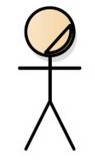
\includegraphics[height=3cm]{Data/actors.png}
      \end{figure}
      \end{column}

  \begin{column}{0.69\textwidth}
    \begin{itemize}
      \item Geographical Information System (GIS)
      \item Grid Operation Scheduler (GOS)
      \item Weather Forecast (WF)
      \item Reserve Aggregator (RA)
      \item Energy Forecaster (EF)
      \item Transmission System Operator (TSO)
      \item Distribution System Operator (DSO)
      \item Transmission Management System (TMS)
      \item Distribution Management System (DMS)
    \end{itemize}
      \end{column}

    \end{columns}

  \end{frame}

  \begin{frame}{Business and function layer}


\begin{figure}[!htb]\centering
  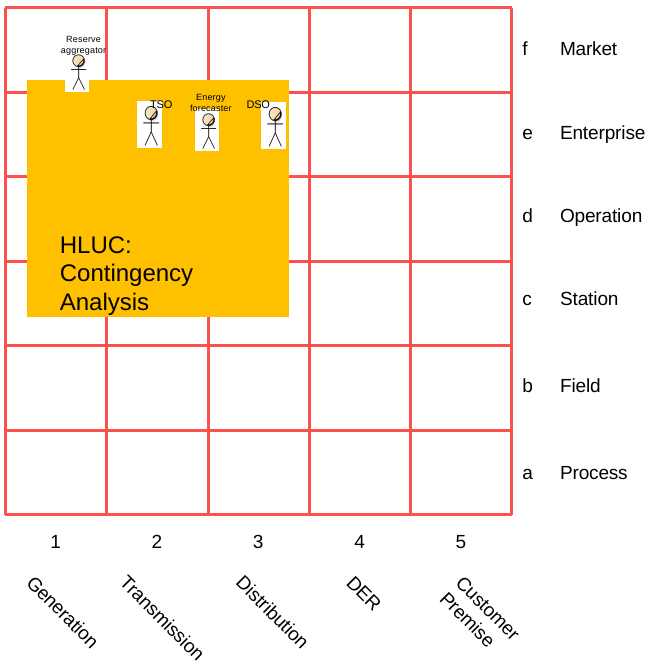
\includegraphics[width=6.0cm]{Data/business.png}
  \hspace{0.1cm}
  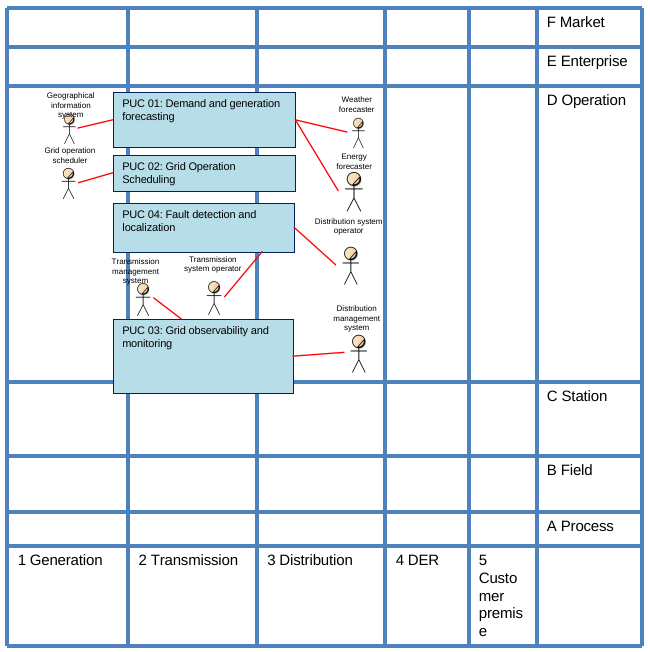
\includegraphics[width=6.0cm]{Data/function.png}
\caption{Business and function layer mapping}
\label{fig:functs}
\end{figure}

  \end{frame}


  \section{Conclusions}
  \begin{frame}{Conclusions}
    \begin{itemize}
      \item The initial grid needs improvements to reduce voltage drops and lines loadings.
        \item A methodology to include new lines is critical. An algorithm to compute the contingencies has been presented.
          \item More lines connecting with the bus of interconnection are required.
          \item Installing renewables has a minor impact on the final results (although they improve).
            \item The storage unit and the dismantled power plant reduce the needs of additional lines.
              \item The high level use case regarding contingencies has been described following the SGAM methodology.
    \end{itemize}
  \end{frame}

  \section{Extra}
  \begin{frame}{Tools}
    \begin{itemize}
      \item Full writing in \LaTeX.
      \item Learning of Python and packages such as \texttt{pandapower} and \texttt{pandas}.
      \item Collaborative work with Git:
    \end{itemize}
    \begin{figure}
      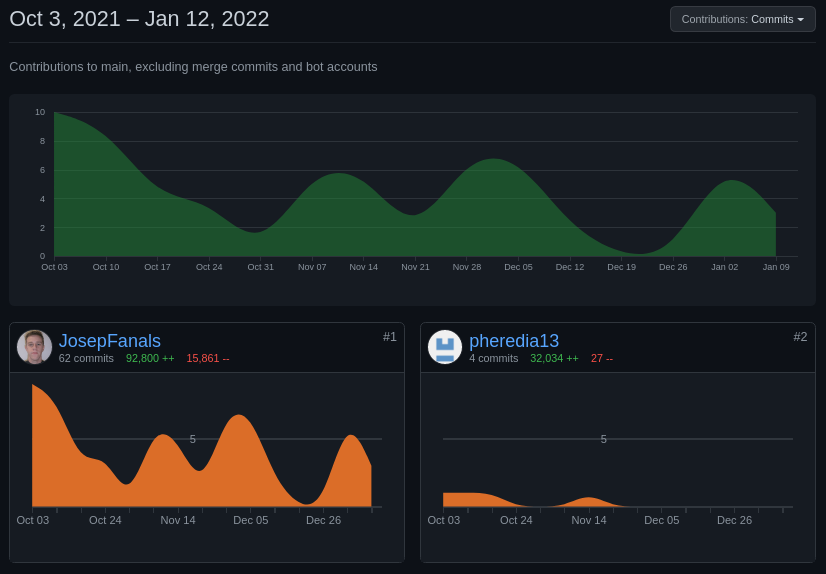
\includegraphics[width=8cm]{Data/git.png}
      \caption{GitHub commits history}
    \end{figure}

  \end{frame}


  \begin{frame}{Workload distribution}
    \begin{itemize}
      \item Víctor: Phase 1 results identification, SGAM
      \item Josep: full Python code, results extraction for all phases, report writing, presentation
      \item Pol: initial Python code, renewables sizing, SGAM
      \item Roger: Phase 1 results identification, Phase 4, SGAM, writing corrections
      \item Palina: Phase 1 results identification, introduction, writing corrections, supervision
    \end{itemize}

  \end{frame}
